\documentclass[14pt]{scrartcl}

\usepackage[utf8]{inputenc}
\usepackage{amsmath,amssymb,amsthm}
\usepackage[croatian]{babel}
\usepackage{csquotes}
\MakeOuterQuote{"}

\usepackage{tikz}
\usetikzlibrary{math}
\newlength{\grlen}
\def\gratio{1.61803}

\usepackage{thmtools}
\usepackage{biblatex}
\addbibresource{literatura.bib}
\usepackage{graphicx}
\graphicspath{ {./images/} }
\usepackage{xcolor}
\usepackage{array}
\usepackage{epigraph}
\usepackage{miama}

\declaretheorem{teorem}
\declaretheorem[sibling=teorem]{korolar}
\declaretheorem[sibling=teorem]{propozicija}
\declaretheorem[name=Primjer,sibling=teorem,qed=$\vartriangleleft$]{primjer}
\declaretheorem[style=definition,sibling=teorem]{definicija}
\declaretheorem[style=remark,sibling=teorem]{napomena}

\usepackage{xparse}
\ExplSyntaxOn
\cs_new:Npn \fibo #1 { \fibo_recurrence:nnnn{0}{1}{0}{#1} }
\cs_new:Npn \fibo_recurrence:nnnn #1 #2 #3 #4
 {
  \int_compare:nTF { #1 = #4 }
  { #3 }
  {
   #3 ~ \fibo_recurrence:ffnn
      { \int_eval:n {#1+1} }
      { \int_eval:n {#2+#3} }
      { #2 }
      { #4 }
  }
 }
\cs_generate_variant:Nn \fibo_recurrence:nnnn { ffnn }
\ExplSyntaxOff

\newcommand{\divfibo}[1]{\frac{#1}{F\sb{n}}}

\begin{document}
\title{FIBONACCIJEVI BROJEVI}
\author{ Mihaela Gamulin}
\date{{\normalsize5. lipnja 2018.}}
\maketitle
\vfill
\epigraph{\fontfamily{qcr}\selectfont\fmmfamily
{\Large"The Fibonacci Sequence turns out to be the key to understanding how nature designs. And is a part of the same ubiquitous music of the spheres that builds harmony into atoms, molecules, crystals, shells, suns and galaxies and makes the Universe sing."}}{\textit{Guy Murchie, \\ The Seven Mysteries of Life}}
\newpage

\tableofcontents
\vspace{5mm}

%-----------------------------------------------------------------------------------------------
\newpage
\section{Uvod}
\line(1,0){500}
\vspace{10mm}
Fibonaccijev niz brojeva jedan je od najpoznatijih nizova brojeva u svijetu. Ime je dobio po matemati\v{c}aru srednjeg vijeka, talijanu Leonardu Pisanu, koji je poznatiji pod imenom (poga\dj{}ate) Fibonacci.\\
Pri\v{c}a je zapo\v{c}ela kada je Pisano postavio matemati\v{c}ki problem razmno\v{z}avanja ze\v{c}eva koji glasi ovako:\\

\hspace{0.5cm}\textit{\enquote{Seljak uzgaja ze\v{c}eve. Svaki par ze\v{c}eva, starih barem dva mjeseca, dobiju svakog mjeseca par mladih: zeca i ze\v{c}icu. Ze\v{c}evi nikad ne umiru. Ako na po\v{c}etku kre\'{c}emo s jednim novoro\dj{}enim parom, koliko će biti ukupno parova ze\v{c}eva nakon n mjeseci?}}\footnote{Pisano je ovaj problem iskazao u svojoj knjizi "Liber Abaccija".}\\

Ako razmislimo o problemu, zaklju\v{c}ujemo da na kraju prvog mjeseca imamo jedan par te na kraju drugog mjeseca tako\dj{}er jedan par. Na kraju tre\'{c}eg mjeseca imamo dva para jer dobivaju dvoje malih ze\v{c}eva. Na kraju \v{c}etvrtog mjeseca seljak ima $2 + 1 = 3$ para. Ako nastavimo istim na\v{c}inom razmi\v{s}ljanja, dobivamo upravo niz:\\

\hspace{3cm} \fibo{15} 
\\

Ovi brojevi su sveprisutni u svijetu, pojavljuju se u geometriji, algebri, teoriji brojeva, \ldots \\
No, \v{s}to je najzanimljivije, pojavljuju se u prirodi i umjetnosti.
I upravo to \v{c}ini matematiku kao znanost još ljep\v{s}om.

%-----------------------------------------------------------------------------------------------
\newpage
\section{Osnovno o Fibonaccijevom nizu}
\line(1,0){500}
\vspace{10mm}

\subsection{Definicije}
\vspace{5mm}

\begin{definicija}\label{opci}
Niz ($F\sb{n}$) zadan je po\v{c}etnim vrijednostima $F\sb{1} = 1$, $F\sb{2} = 1$, te rekurzivnom relacijom
\begin{equation}
F\sb{n+1}=F\sb{n}+F\sb{n-1},
\end{equation}
za sve $n \geq 2$, naziva se \emph{\textbf{Fibonaccijev niz}}. Op\'{c}i \v{c}lan niza $F\sb{n}$ jo\v{s} zovemo \emph{\textbf{n-ti Fibonaccijev broj}}.\\
\end{definicija}

Ponekad inicijaliziramo niz s $F\sb{0}=0$ i $F\sb{1}=1$.
Svaki rekurzivan niz, pa tako i Fibonaccijev, ovisi o zadanim po\v{c}etnim uvjetima.\\

\begin{definicija}\label{generalizirani}
Neka su $a, b\in\mathbb{Z}$. Niz ($G\sb{n}$) zadan po\v{c}etnim vrijednostima $G\sb{0} = a$, $G\sb{1} = b$, te rekurzivnom relacijom
\begin{equation}
G\sb{n+1} = G\sb{n}+G\sb{n-1},
\end{equation}
za $n \geq 1$, naziva se \emph{\textbf{generalizirani Fibonaccijev niz}}.
\end{definicija}

Raspisivanjem prvih nekoliko \v{c}lanova generaliziranog Fibonaccijevog niza 
\begin{gather*}
G\sb{2} = a+b,\\
\quad \! \! \! G\sb{3} = a+2b,\\
\quad G\sb{4} = 2a+3b,\\
\quad G\sb{5} = 3a+5b,\\
\quad G\sb{6} = 5a+8b,\\
\! \! \! \! \! \! \! \! \vdots 
\end{gather*}
uo\v{c}avamo da se kao koeficijenti pojavljuju \v{c}lanovi obi\v{c}nog Fibonaccijevog niza (Definicija \ref{opci}). Vrijedi sljede\'{c}a propozicija:

\begin{propozicija}
Ako je ($G\sb{n}$) generalizirani Fibonaccijev niz odre\dj{}en po\v{c}etnim vrijednostima $G\sb{0} = a$ i $G\sb{1} = b$, onda vrijedi $G\sb{n} = aF\sb{n-1}+bF\sb{n}$, za sve $n\in\mathbb{N}$ i $n \geq 2$.
\end{propozicija}
\newpage
\begin{proof}
Tvrdnju \'{c}emo pokazati pomo\'{c}u matemati\v{c}ke indukcije. Baza vrijedi jer za $n=2$ imamo:
\begin{equation}
G\sb{2} = aF\sb{1}+bF\sb{2} = a+b. \notag
\end{equation}
Pretpostavimo da tvrdnja
\begin{equation}
G\sb{k} = aF\sb{k-1}+bF\sb{k} \notag
\end{equation}
vrijedi za sve $k\in\mathbb{N}$ i $2 \leq k \leq n$. Poka\v{z}imo da tvrdnja vrijedi i za $k = n + 1$:
\begin{multline}
G\sb{n+1}=G\sb{n}+G\sb{n-1}=(P.I.)=aF\sb{n-1}+bF\sb{n}+aF\sb{n-2}+bF\sb{n-1}\\
=a(F\sb{n-1}+F\sb{n-2})+b(F\sb{n}+F\sb{n-1})=aF\sb{n}+bF\sb{n+1} \notag
\end{multline}
\end{proof}

\subsection{Binetova formula}\label{binet}
\vspace{5mm}

Binet je 1843.~godine izveo formulu za eksplicitno ra\v{c}unanje Fibonaccijevih brojeva te je ona dana sljede\'{c}im teoremom:

\begin{teorem}\label{tm:binet}
\textbf{(Binetova formula za Fibonaccijeve brojeve)}\\
Vrijedi
\begin{equation}\label{eq:binet}
F\sb{n}=\frac{1}{\sqrt[]{5}}\Bigl(\Bigl(\frac{1+\sqrt[]{5}}{2}\Bigr)\sp{n}-\Bigl(\frac{1-\sqrt[]{5}}{2}\Bigr)\sp{n}\Bigr), 
\end{equation}
za sve $n \geq 1$.\\
\end{teorem}

Tako\dj{}er vrijede i sljede\'{c}i identiteti: (za ostale pogledati \cite{dujella} i \cite{wiki}).

\begin{propozicija}
Vrijedi
\begin{equation}
F\sb{m+n}=F\sb{m}F\sb{n+1}+F\sb{m-1}F\sb{n},
\end{equation}
za sve $n, m \geq 1$.\\
\end{propozicija}

\begin{propozicija}
Vrijedi
\begin{equation}
F\sb{1}+F\sb{2}+\dots+F\sb{n}=F\sb{n+2}-1,
\end{equation}
za $n \geq 0$.
\end{propozicija}
\begin{proof}
Formulu dobivamo zbrajanjem sljede\'{c}ih osnovnih relacija
\begin{gather*}
F\sb{1} = F\sb{3}-F\sb{2},\\
F\sb{2} = F\sb{4}-F\sb{3},\\
\! \! \! \! \! \! \! \! \! \! \! \! \! \! \! \vdots\\
F\sb{n-1} = F\sb{n+1}-F\sb{n},\\
\qquad \! F\sb{n} = F\sb{n+2}-F\sb{n+1}.
\end{gather*}
\end{proof}

\begin{primjer}
Kvadrati Fibonaccijevih brojeva \v{c}ine zanimljivu shemu:
\begin{align}
1\sp{2}+1\sp{2}=1\cdot2\notag\\
1\sp{2}+1\sp{2}+2\sp{2}=2\cdot3\notag\\
1\sp{2}+1\sp{2}+2\sp{2}+3\sp{2}=3\cdot5\notag\\
1\sp{2}+1\sp{2}+2\sp{2}+3\sp{2}+5\sp{2}=5\cdot8\notag\\
1\sp{2}+1\sp{2}+2\sp{2}+3\sp{2}+5\sp{2}+8\sp{2}=8\cdot1&3\notag
\end{align}
\end{primjer}

\subsection{Djeljivost}
\vspace{5mm}

Fibonaccijevi brojevi su prirodni brojevi pa na njima mo\v{z}emo promatrati djeljivost.
Najve\'{c}u zajedni\v{c}ku mjeru prirodnih brojeva a i b u daljnjem razmatranju ozna\v{c}avamo
\begin{equation}
(a,b) \notag \\
\end{equation}

\begin{propozicija}
Svaka dva uzastopna Fibonaccijeva broja su relativno prosti.
\end{propozicija}
\begin{napomena}
Brojevi $a$ i $b$ su relativno prosti ako je njihov najve\'{c}i zajedni\v{c}ki djelitelj jednak $1$, tj. brojevi $a$ i $b$ nemaju zajedni\v{c}kih faktora.
\end{napomena}
\begin{proof}
Za $n\in\mathbb{N}$, stavimo $d=(F\sb{n},F\sb{n+1})$. Kako $d$ dijeli $F\sb{n}$ i $F\sb{n+1}$, onda $d$  dijeli i 
\begin{equation}
F\sb{n+1}-F\sb{n}=F\sb{n-1}.\notag
\end{equation}
Dalje, zaklju\v{c}ujemo da $d$ dijeli redom
\begin{equation}
F\sb{n}-F\sb{n-1}=F\sb{n-2},\; F\sb{n-1}-F\sb{n-2}=F\sb{n-3},\;\ldots,\; F\sb{3}-F\sb{2}=F\sb{1}=1.\notag
\end{equation}
Vidimo $d=1$, \v{s}to je trebalo i dokazati.
\end{proof}

\begin{propozicija}\label{propdijeli}
Neka su $m$ i $n$ prirodni brojevi. Ako $n$ dijeli $m$, onda $F\sb{n}$ dijeli $F\sb{m}$.
\end{propozicija}

\begin{korolar}\label{korolarsloz}
Ako je $n$ slo\v{z}en prirodan broj razli\v{c}it od 4, onda je $F\sb{n}$ slo\v{z}en broj.
\end{korolar}
\begin{proof}
Ako je broj $n$ slo\v{z}en, onda se on mo\v{z}e zapisati u obliku $n=ab$, gdje su $a,b>1$. Kako je $n \neq 4$, to je bar jedan od brojeva $a$ i $b$ ve\'{c}i od $2$. Recimo da je $a>2$. Tada je $F\sb{a} \neq F\sb{n}$ i $F\sb{n} \neq 1$, a prema Propoziciji \ref{propdijeli} znamo da je $F\sb{a} \mid F\sb{n}$. To zna\v{c}i da je $F\sb{n}$ slo\v{z}en.
\end{proof}

\begin{primjer}
Obrat tvrdnje iz Korolara \ref{korolarsloz} ne vrijedi.
Naime mo\v{z}e se dogoditi da je broj $p$ prost, a da je broj $F\sb{p}$ slo\v{z}en. Na primjer: $F\sb{19} = 4181 = 37 \cdot 113$.
\end{primjer}

%------------------------------------------------------
\newpage
\section{Zlatni rez i Fibonaccijevi brojevi}
\line(1,0){500}
\vspace{10mm}

Zlatni rez~\cite{wiki} je pojam koji ljudi naj\v{c}e\v{s}\'{c}e ve\v{z}u uz pojam sklada, savr\v{s}enstva i ravnote\v{z}e.\\
\[
  \setlength{\grlen}{100pt}
  \underbrace{%
    \overbrace{
      \makebox[0pt][l]{\rule[-1ex]{.4pt}{2.4ex}}
      \makebox[\gratio\grlen]{\hrulefill}
      \makebox[0pt][r]{\rule[-1ex]{.2pt}{2.4ex}}}^x
    \mkern-3mu
    \overbrace{
      \makebox[0pt][l]{\rule[-1ex]{.2pt}{2.4ex}}
      \makebox[\grlen]{\hrulefill}
      \makebox[0pt][r]{\rule[-1ex]{.4pt}{2.4ex}}}^y
  }_{x+y}
\]
Pi\v{s}emo:
\\
\begin{equation}
\frac{x+y}{x}=\frac{x}{y}=\varphi \\
\end{equation}
Dakle, zlatni rez $\varphi$ je pozitivno rje\v{s}enje kvadratne jednad\v{z}be\\
\begin{equation}
x\sp{2}-x-1=0 \\
\end{equation}
koja se naziva zlatna jednad\v{z}ba te njen rezultat iznosi\\
\begin{equation}
\varphi=\frac{1+\sqrt[]{5}}{2}\approx 1.61803398 \dots
\end{equation}
\\Pitamo se, naravno, kakve veze ima zlatni rez s Fibonaccijevim brojevima. U tu svrhu promotrimo tablicu u kojoj su dani omjeri susjednih Fibonaccijevih brojeva:
\renewcommand{\arraystretch}{2}
\begin{center}
 \begin{tabular}{| c |}
 \hline
 $\divfibo{F\sb{n+1}}$ \\
 \hline\hline
 $\frac{2}{1}=2.000000$\ldots \\
 \hline
 $\frac{3}{2}=1.500000$\ldots \\ 
 \hline
 $\frac{5}{3}=1.666666$\ldots \\ 
 \hline
 \vdots \\ 
 \hline
 $\frac{987}{610}=1.618033$\ldots \\ 
 \hline
 $\frac{1597}{987}=1.618034$\ldots \\
 \hline 
\end{tabular} 
\end{center}
\newpage
Iz ovog primjera mo\v{z}emo naslutiti da niz ($F\sb{n+1}/F\sb{n}$) konvergira upravo zlatnom rezu. 
Fascinantno,zar ne?\\ \\
Koriste\'{c}i Binetovu formulu (\ref{eq:binet}) iz odjeljka \ref{binet}, Teorem \ref{tm:binet}, dobivamo:\\
\begin{equation}
\lim_{n\to\infty}\divfibo{F\sb{n+1}}=\lim_{n\to\infty}\frac{\frac{1}{\sqrt[]{5}}(\alpha\sp{n+1}-\beta\sp{n+1})}{\frac{1}{\sqrt[]{5}}(\alpha\sp{n}-\beta\sp{n})}=\lim_{n\to\infty}\frac{\alpha-\beta(\beta/\alpha)\sp{n}}{1-(\beta/\alpha)\sp{n}}=\alpha=\varphi
\end{equation}
\\jer je $\frac{\beta}{\alpha}$ po apsolutnoj vrijednosti manja od $1$ pa to povla\v{c}i da
\begin{equation}
\lim_{n\to\infty}\Bigl(\frac{\beta}{\alpha}\Bigr)\sp{n}=0. \notag
\end{equation}
\\
Zna\v{c}i li to da su i Fibonaccijevi brojevi savr\v{s}eni i u skladu? To ostavljam \v{c}itatelju da odlu\v{c}i, a u daljnjem nastavku vidjet \'{c}emo samo mali dijeli\'{c} pojave tih intrigantnih brojeva.

%------------------------------------------------------
\newpage
\section{Fibonaccijevi brojevi u umjetnosti}
\line(1,0){500}
\vspace{10mm}

Svi danas te\v{z}imo ljepoti. Dok drugi te\v{z}e nekim drugim ljepotama, mi matemati\v{c}ari tra\v{z}imo ljepotu u brojevima i formulama. Jo\v{s} od ranih vremena tra\v{z}ila se univerzalna matemati\v{c}ka formula ljepote, koja je prona\dj{}ena upravo u zlatnom omjeru, a ovdje  \'{c}e nam poslu\v{z}iti kao most prema Fibonaccijevim brojevima.
\\

Mnogi veliki umjetnici, još od Stare Gr\v{c}ke, sakrili su u svojim djelima taj sklad proporcija.
Ja \'{c}u se u ovom radu okrenuti jednom od najve\'{c}ih ljudi tog vremena, ako ne i svih vremena. 
Poga\dj{}ate o kome je rije\v{c}?\\

Leonardo da Vinci, poznati talijanski slikar, kipar, arhitekt, znanstvenik i in\v{z}injer, zapravo renesansni \v{c}ovjek, u svojim je djelima te\v{z}io savr\v{s}enstvu.
On je u svojem Vitruvijevom \v{c}ovjeku pokazao kako su proporcije ljudskog tijela skoro pa savr\v{s}ene te kako te proporcije trebaju biti osnova arhitekture. Konstruirao je proporciju ljudskog tijela na osnovi zlatnog reza kao \v{s}to je prikazano na Slici \ref{fig:vitruvi}.\\
\begin{figure}[hb!]
\begin{center}
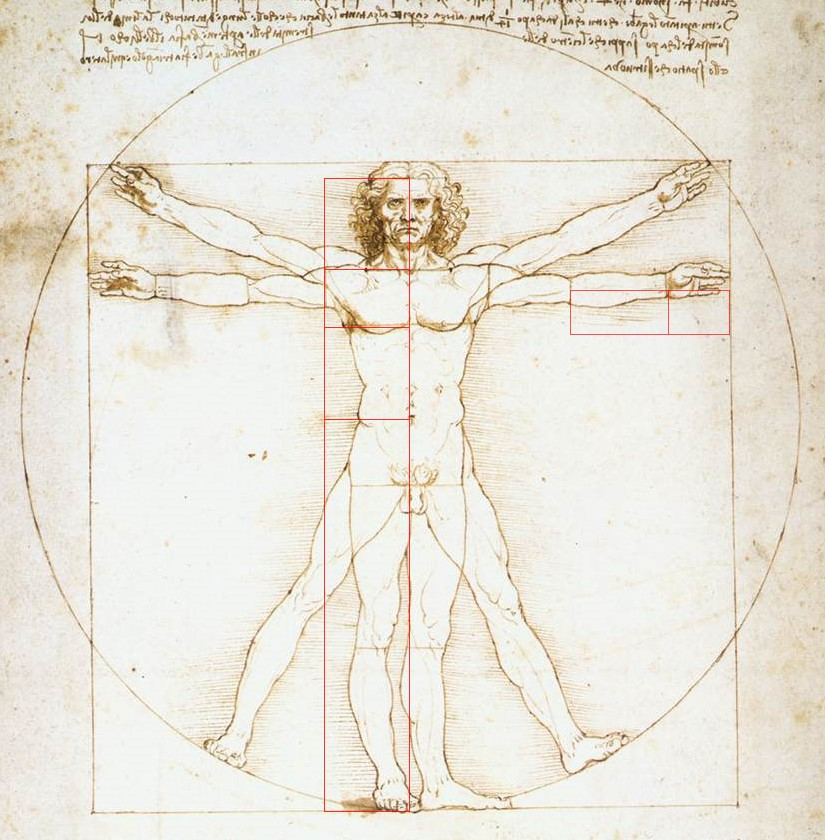
\includegraphics[scale=0.5]{Vitruvi.jpg}
\end{center}
\caption{Slika Vitruvijevog čovjeka}
\label{fig:vitruvi}
\end{figure}
\newpage
Crte\v{z} nam ka\v{z}e da je ljudsko tijelo mogu\'{c}e ucrtati u kru\v{z}nicu i kvadrat. Visina \v{c}ovjeka jednaka je \v{s}irini rastvorenih ruku, a postavljanjem ruku i nogu u dijagonalu \v{c}ovjek postaje sredi\v{s}te kru\v{z}nice. Potezi ispod koljena ozna\v{c}avaju zlatni rez kao i na ramenima: od vrha prstiju do ramena, rame do prstiju druge ruke.\\

Iako postoji bezbroj primjera iz proteklih nekoliko stolje\'{c}a me\dj{}u kojima bi se mogle na\'{c}i pojave zlatnog reza, odnosno Fibonaccijevih brojeva, zadr\v{z}at \'{c}emo se opet na da Vinciju i jednoj od zasigurno najpoznatijih slika zapadne umjetnosti, a to je \v{c}uvena Mona Lisa.\\
\begin{figure}[hb!]
\begin{center}
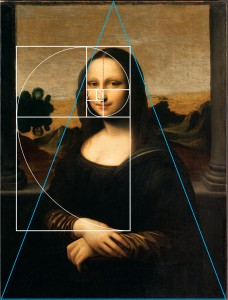
\includegraphics[scale=0.7]{MonaLisa.jpg}
\end{center}
\caption{Slika Mona Lise}
\label{fig:mona}
\end{figure}

Ovu sliku progla\v{s}avaju jednom od najboljih remek-dijela svih vremena. I tu mo\v{z}emo primjetiti igru zlatnog reza.\\

Kako nebi mislili da se samo u slikama mo\v{z}e prona\'{c}i ravnote\v{z}a, pokazat \'{c}emo i jedan primjer u arhitekturi.
Naime tijekom renesanse, nacrti mnogih gra\dj{}evinskih projekata koristili su Fibonaccijeve brojeve ili zlatni omjer. Mo\v{z}e ih se prona\'{c}i,na primjer, na nacrtima kupole katedrale Santa Maria del Fiore u Firenci koja se mo\v{z}e vidjeti na Slici \ref{fig:kupola}. Skica \footnote{Gruba skica Giovannija di Gherarda da Pratoa (1426.), dok je za konstrukciju zaslu\v{z}an Fillippo Brunelleschi.} kupole pokazuje Fibonaccijeve brojeve: 55, 89 i 144 te brojeve 17 (\v{s}to je polovica Fibonaccijevog broja 34) i 72 (\v{s}to je polovica Fibonaccijevog broja 144).\\
\newpage
\begin{figure}[hb!]
\begin{center}
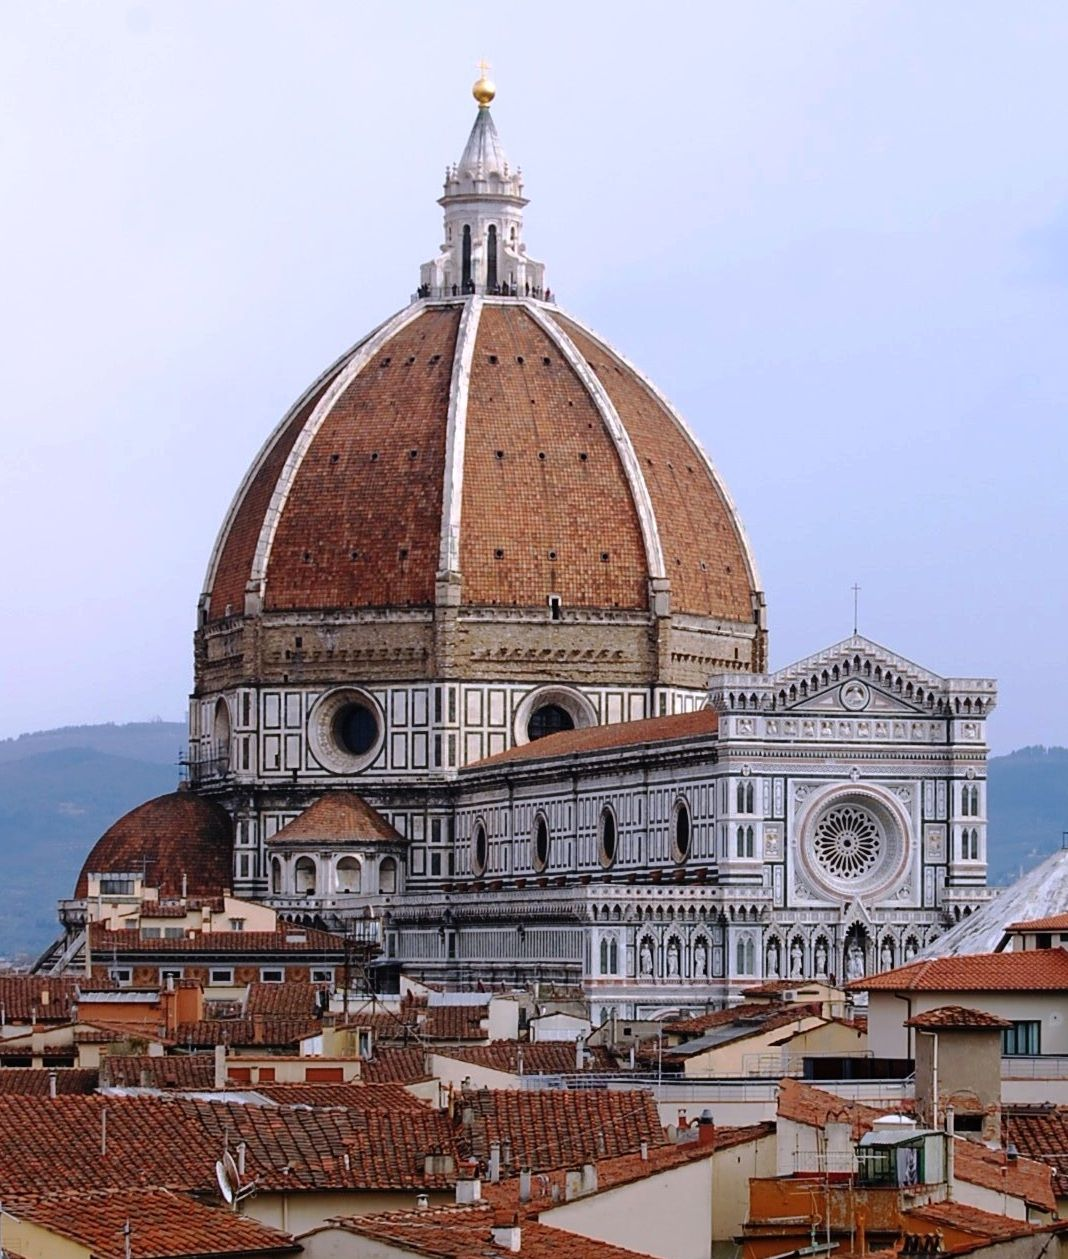
\includegraphics[scale=0.4]{Kupola.jpg}
\end{center}
\caption{Slika kupole katedrale Santa Maria del Fiore u Firenci, Italija}
\label{fig:kupola}
\end{figure}

%------------------------------------------------------
\newpage
\section{Fibonaccijevi brojevi u prirodi}
\line(1,0){500}
\vspace{5mm}

\begin{enumerate}
\item Suncokret:
Pogledajte red sjemena u centru suncokreta i primjetit \'{c}ete ne\v{s}to \v{s}to izgleda kao spiralni uzorak. Ako prebrojite te sprale dobit ćete Fibonaccijev broj.
\item Cvije\'{c}e: 
Ako prebrojite latice na nekom cvijetu, suma \'{c}e vrlo \v{c}esto biti jedan od brojeva Fibonaccijevog niza.\cite{nature}
\item Ljudsko tijelo: Pogledajte se u ogledalo i vidjet \'{c}ete Fibonaccijev niz. Va\v{s}e tijelo se sastoji od brojeva 1, 2, 3 i 5. Imate jedan nos, dva oka, tri segmenta svakog ud-a i pet prstiju na svakoj ruci. Izmjerimo li du\v{z}inu \v{c}ovjeka od vrha glave do poda, zatim to podijelimo s du\v{z}inom od pupka do poda dobijemo $1.618034$.
\item Oklop Nutilus-a: Jedan od najpoznatijih primjera Fibonaccijeve spirale je oklop glavono\v{s}ca Nutilus-a kojeg smo svi vidjeli bar jednom kao naslovnu sliku knjige o geometriji. Fibonaccijeva spirala stvorena je iscrtavanjem lukova koji spajaju suprotne kuteve kvadrata u Fibonaccijevom poplo\v{c}anju. Ta spirala je temeljena na progresiji Fibonaccijevog niza. Kad bi izra\v{c}unali odnos svakog spiralnog promjera dobili bismo upravo zlatni rez.\\

\begin{figure}[hb!]
\begin{center}
\def\spiral#1{%
  \pgfmathparse{int(#1)}%
  \ifnum\pgfmathresult>0
    \draw [help lines] (0,0) rectangle ++(1,1);
    \begin{scope}[shift={(1,1)}, rotate=90, scale=1/1.6180339887]
      \spiral{#1-1}
    \end{scope}
    \draw [red] (0,0) arc (270:360:1);
  \fi
}
\tikz[scale=5]{\spiral{12}}
\end{center}
\caption{Slika Fibonaccijeve spirale}
\label{fig:spirala}
\end{figure}
\end{enumerate}
 
\newpage
\section{Literatura i popis slika}
\line(1,0){500}
\vspace{10mm}

\printbibliography
\listoffigures

\end{document}